\begin{tikzpicture}
    \node[anchor=south west] (image1) at (0,0) {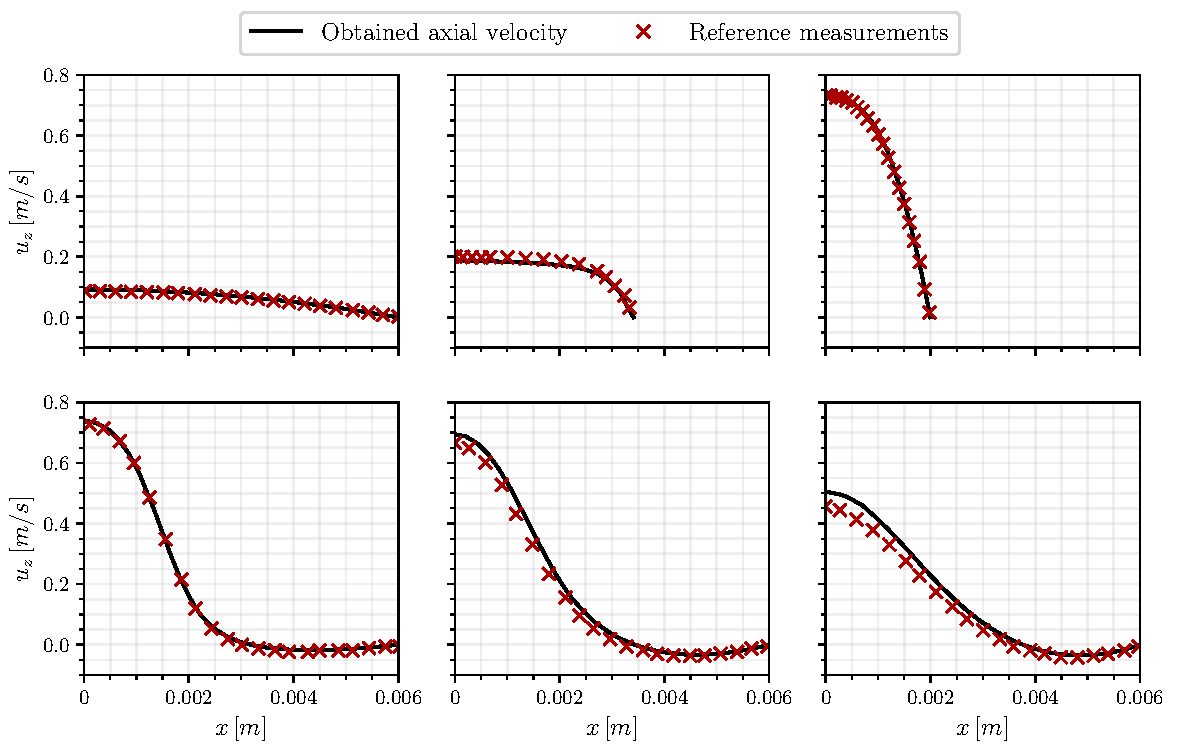
\includegraphics[width=\linewidth]{chapter2/Figures/FDA/Re500/radial_velocities.pdf}};
    \node[anchor=north west, xshift=1.85cm, yshift=-1.2cm] (image2) at (image1.north west) {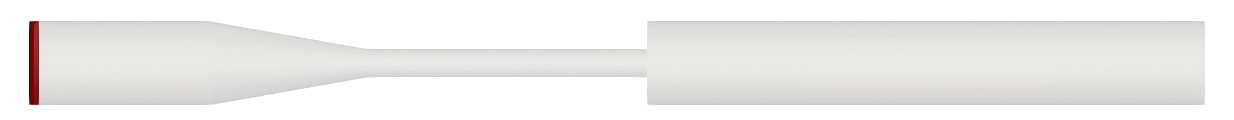
\includegraphics[width=0.2\linewidth]{chapter2/Figures/FDA/-88.png}};
    \node[anchor=north west, xshift=6.5cm, yshift=-1.2cm] (image2) at (image1.north west) {
\includegraphics[width=0.2\linewidth]{chapter2/Figures/FDA/-48.png}};
    \node[anchor=north west, xshift=11.1cm, yshift=-1.2cm] (image2) at (image1.north west) {
\includegraphics[width=0.2\linewidth]{chapter2/Figures/FDA/-8.png}};
    \node[anchor=north west, xshift=1.85cm, yshift=-5.3cm] (image2) at (image1.north west) {
\includegraphics[width=0.2\linewidth]{chapter2/Figures/FDA/8.png}};
    \node[anchor=north west, xshift=6.5cm, yshift=-5.3cm] (image2) at (image1.north west) {
\includegraphics[width=0.2\linewidth]{chapter2/Figures/FDA/24.png}};
    \node[anchor=north west, xshift=11.1cm, yshift=-5.3cm] (image2) at (image1.north west) {
\includegraphics[width=0.2\linewidth]{chapter2/Figures/FDA/80.png}};
\end{tikzpicture}